\documentclass[a4paper,titlepage,halfparskip,12pt]{scrreprt}
\usepackage[ngerman]{babel, varioref}
\usepackage[utf8]{inputenc}
\usepackage[T1]{fontenc}
\usepackage{graphicx}
\usepackage{fancyhdr}
\usepackage{amsmath}
\usepackage{geometry}
\geometry{a4paper, top=25mm,left=25mm,right=25mm,bottom=25mm, footskip=12mm}
\usepackage{longtable}
\usepackage{setspace}
\usepackage{lmodern}
%blocksatz
\sloppy
%formatierung literaturverzeichnisangabe
\bibliographystyle{unsrt}

%Auflistungen von Punkten
\usepackage{paralist} 
%urls anzeigen
\usepackage{url}

\usepackage{notoccite}

%Codelisting
\usepackage{xcolor}
\definecolor{mygreen}{rgb}{0,0.6,0}
\definecolor{mygray}{rgb}{0.5,0.5,0.5}
\definecolor{mymauve}{rgb}{0.58,0,0.82}
\definecolor{burntorange}{rgb}{0.8, 0.33, 0.0}
\definecolor{cornellred}{rgb}{0.7, 0.11, 0.11}


\usepackage{listingsutf8}
\lstset{
commentstyle=\color{mygreen},
numberstyle=\small\color{black},
stringstyle=\color{mymauve},
emph={square}, 
showstringspaces=false,
flexiblecolumns=false,
tabsize=2,
numbers=left,
numberblanklines=false,
stepnumber=1,
captionpos=b,
numbersep=5pt,
xleftmargin=15pt,
breaklines=true,
inputencoding=utf8,
extendedchars=true,
extendedchars=true,
basicstyle=\ttfamily\footnotesize,
keywordstyle = \bfseries\color{burntorange},
keywordstyle = [2]\bfseries\color{cornellred},
literate=%
    {Ä}{{\"A}}1%
    {Ö}{{\"O}}1%
    {Ü}{{\"U}}1%
    {ä}{{\"a}}1%
    {ö}{{\"o}}1%
    {ü}{{\"u}}1%
    {ß}{{\ss}}1,%
frame=single,
frameround=ffff
}

%define Javascript language
\lstdefinelanguage{JavaScript}{
	keywords={typeof, new, true, false, catch, function, return, null, catch, switch, var, if, in, while, do, else, case, break},
	keywordstyle=\color{blue}\bfseries,
	ndkeywords={class, export, boolean, throw, implements, import, this},
	ndkeywordstyle=\color{darkgray}\bfseries,
	identifierstyle=\color{black},
	sensitive=false,
	comment=[l]{//},
	morecomment=[s]{/*}{*/},
	commentstyle=\color{purple}\ttfamily,
	stringstyle=\color{red}\ttfamily,
	morestring=[b]',
	morestring=[b]"
}

%% start defining yaml listings layout
\newcommand\YAMLcolonstyle{\color{red}\mdseries}
\newcommand\YAMLkeystyle{\color{black}\bfseries}
\newcommand\YAMLvaluestyle{\color{blue}\mdseries}

\makeatletter

% here is a macro expanding to the name of the language
% (handy if you decide to change it further down the road)
\newcommand\language@yaml{yaml}

\expandafter\expandafter\expandafter\lstdefinelanguage
\expandafter{\language@yaml}
{
  keywords={true,false,null,y,n},
  keywordstyle=\color{blue}\bfseries,
  basicstyle=\YAMLkeystyle,                                 % assuming a key comes first
  sensitive=false,
  comment=[l]{\#},
  morecomment=[s]{/*}{*/},
  commentstyle=\color{mygreen}\ttfamily,
  stringstyle=\YAMLvaluestyle\ttfamily,
  moredelim=[l][\color{orange}]{\&},
  moredelim=[l][\color{magenta}]{*},
  moredelim=**[il][\YAMLcolonstyle{:}\YAMLvaluestyle]{:},   % switch to value style at :
  morestring=[b]',
  morestring=[b]",
  literate =    {---}{{\ProcessThreeDashes}}3
                {>}{{\textcolor{red}\textgreater}}1     
                {|}{{\textcolor{red}\textbar}}1 
                {\ -\ }{{\mdseries\ -\ }}3,
}

% switch to key style at EOL
\lst@AddToHook{EveryLine}{\ifx\lst@language\language@yaml\YAMLkeystyle\fi}
\makeatother

\newcommand\ProcessThreeDashes{\llap{\color{cyan}\mdseries-{-}-}}

% end defining yaml listings layout

%meta data
\usepackage[hidelinks]{hyperref}
\urlstyle{same}

%akronymverzeichnis
\usepackage[printonlyused]{acronym}

% titel definieren
\newcommand{\titel}{Entwicklung eines Chatsystems\\auf Basis von XMPP}

%autor definieren
\newcommand{\autor}{Lukas Priester,Oliver Klapper}
\newcommand{\keywords}{\autor,\titel,Studienarbeit}

% Allgemeines für das PDF
\hypersetup{
    pdftitle={\titel},
    pdfauthor={\autor},
    pdfcreator={\autor},
    pdfsubject={\titel},
    pdflang={Deutsch},
    pdfdisplaydoctitle=true,
    pdfkeywords={\keywords},
}

% set distances of chapter headlines in document
\renewcommand*\chapterheadstartvskip{\vspace*{20pt}} % set distance to header
% set distance to text
%\renewcommand*\chapterheadendvskip{%
%  \vspace*{1\baselineskip plus .1\baselineskip minus .167\baselineskip}}

%TODO überall eigene Darstellung unter Abbildungen hinzufügen

\begin{document}

\begin{table}[h]
\centering
\begin{tabular}{lcr}
\end{tabular}
\end{table}
\bigskip
\bigskip
\begin{center}
\vspace*{12mm} {\LARGE\textbf{\titel}}\\
\vspace*{12mm} {\large\textbf{Studienarbeit}}\\
\vspace*{3mm} {\large\textbf{5. - 6. Semester}}\\
\vspace*{12mm} des Studiengangs Informationstechnik (B.Sc.)\\ an der Dualen Hochschule Baden-Württemberg Stuttgart\\
% \vspace*{3mm} an der Dualen Hochschule Baden-Württemberg\\
\vspace*{12mm} von\\
\vspace*{3mm} {\large\textbf{Lukas Priester, Oliver Klapper}}\\
\vspace*{12mm} \today\\
\end{center}
\vfill
\begin{spacing}{1.5}
\begin{tabbing}
mmmmmmmmmmmmmmmmmmmmmmmmmm \= \kill
\textbf{Bearbeitungszeitraum} \> 01.10.2019 - 01.05.2020\\
\textbf{Matrikelnummer, Kurs} \> 7288057, 4191693 \\
\textbf{Kurs} \> TINF17IN\\
\textbf{Betreuer der Hochschule} \> Alfred Becker\\
\textbf{Gutachter der Hochschule} \> Alfred Becker\\
\end{tabbing}
\end{spacing}
%Seitennummerierung ausschalten
\pagenumbering{gobble}
\newpage

\section*{Selbstständigkeitserklärung}

\bigskip

Ich versichere hiermit, dass ich meine Bachelorarbeit (bzw. Studien- und Projektarbeit) mit dem Thema:

\smallskip

%% eigentlich hier \titel verwenden statt duplicated titel, aber umbruch erzwingt
%% doppeltes ausschreiben des titels
\texttt{Entwicklung eines Chatsystems auf Basis von XMPP}

\smallskip

selbstständig verfasst und keine anderen als die angegebenen Quellen und Hilfsmittel benutzt habe.

\bigskip

Ich versichere zudem, dass die eingereichte elektronische Fassung mit der gedruckten Fassung übereinstimmt.*

\bigskip

\begin{small}

* falls beide Fassungen gefordert sind

\bigskip

\bigskip

\noindent\begin{tabular}{ll}
\makebox[2.5in]{\hrulefill} & \makebox[2.5in]{\hrulefill}\\
Ort, Datum & Unterschrift
\end{tabular}
\end{small}

\newpage

%abstract text
\section*{Abstract}

\newpage

%inhaltsverzeichnis
	% Inhaltsverzeichnis
	\cleardoublepage
	\begin{spacing}{1.1}
		\begingroup
		
			% auskommentieren für Seitenzahlen unter Inhaltsverzeichnis
			\renewcommand*{\chapterpagestyle}{empty}
			\pagestyle{empty}
			
			
			%\setcounter{tocdepth}{1}
			%für die Anzeige von Unterkapiteln im Inhaltsverzeichnis
			\setcounter{tocdepth}{2}
			
			\tableofcontents
			\clearpage
		\endgroup
	\end{spacing}

%% new header/footer settings
\renewcommand{\sectionmark}[1]{\markright{\thesection\ #1}} % make header rightmark
\fancypagestyle{fancyheadlines}{
\pagenumbering{arabic}
\fancyhf{}
\lhead{\slshape\rightmark}
%%\rhead{\slshape\nouppercase{\leftmark}}
\renewcommand{\headrulewidth}{0.4pt}
%\lfoot{\slshape DHBW Stuttgart | Lukas Priester, Oliver Klapper}
\cfoot{\thepage}
\renewcommand{\footrulewidth}{0.4pt}
}

% Redefine the plain page style, show only page number in figure,table,...contents
% and chapter pages
\fancypagestyle{plain}{%
  \fancyhf{}%
  %\lfoot{\slshape DHBW Stuttgart | Lukas Priester, Oliver Klapper}%
  \cfoot{\thepage}
  \renewcommand{\headrulewidth}{0pt}% Line at the header invisible
  \renewcommand{\footrulewidth}{0.4pt}% Line at the footer visible
}


\newpage
\pagenumbering{Roman}


%abkürzungsverzeichnis
\cleardoublepage
\addcontentsline{toc}{chapter}{Abkürzungsverzeichnis}
\chapter*{Abkürzungsverzeichnis}
\begin{acronym}[YTMMM]
\setlength{\itemsep}{-\parsep}

\acro{IMS} {Instant Messaging System}
\acro{XMPP} {Extensible Messaging and Presence Protocol}
\acro{XML} {Extensible Markup Language}
\acro{TCP} {Transmission Control Protocol}
\acro{TLS} {Transport Layer Security}
\acro{MUC} {Multi-User-Chat}
\acro{NLP} {Natural Language Processing}
\acro{MUC} {Multi User Chat}
\acro{ICQ} {I seek you}
\acro{VoIP} {Voice over IP}
\acro{HTML}{HyperText Markup Language}
\acro{DBMS}{Datenbankenmanagementsystem}
\acro{SQL}{Structured Query Language}
\acro{GUI}{graphical user interface}
\acro{WSGI}{Web Server Gateway Interface}
\acro{CSS}{Cascading Style Sheets}
\acro{Ajax}{Asynchronous JavaScript and XML}
\acro{ORM}{Object Relational Mapper}
\acro{CA}{Certification Authority}
\acro{RSA}{Rivest-Shamir-Adleman}
\acro{BSI}{Bundesamt für Sicherheit in der Informationstechnik}
\acro{PFS}{Perfect Forward Secrecy}
\acro{ACL}{Access Control List}
\acro{YAML}{YAML Ain't Markup Language}
\acro{DNS}{Domain Name System}
\acro{AES}{Advanced Encryption Standard}
\acro{DES}{Data Encryption Standard}
\acro{SSL}{Secure Socket Layer}
\acro{DOS}{Denial of Service}
\acro{URI}{Uniform Resource Identifier}
\acro{SASL}{Simple Authentication and Security Layer}
\acro{RFC}{Request for Comments}
\acro{MD5}{Message Digest Algorithm 5}
\acro{MAM}{Message Archive Management}
\acro{HTTP}{Hypertext Transfer Protocol}
\acro{REST}{Representational State Transfer}
\acro{API}{Application Programming Interface}
\acro{SSH}{Secure Shell}
\acro{HTML}{Hypertext Markup Language}
\acro{PDF}{Portable Document Format}
\acro{JSON}{JavaScript Object Notation}
\acro{XML}{Extensible Markup Language}
\acro{JS}{JavaScript}
\acro{DOM}{document object model}
\end{acronym}

%abbildungsverzeichnis
\cleardoublepage
\addcontentsline{toc}{chapter}{\listfigurename}
\listoffigures
\newpage
%tabellenverzeichnis
\cleardoublepage
\addcontentsline{toc}{chapter}{\listtablename}
\listoftables
\newpage
%listingverzeichnis
\cleardoublepage
\addcontentsline{toc}{chapter}{\lstlistingname}
\lstlistoflistings
\newpage

\begin{onehalfspacing}

%% header and footer settings
\pagestyle{fancyheadlines}

\chapter{Einleitung}
\label{chap:Einleitung}



\chapter{Umsetzung und Implementierung}
\label{chap:Umsetzung}

%%%%%%%%%%%%%%%%%%%%%%%%%%%%%%%%%%%%%%%%%%%%%%%%%%%%
%%%%%%%%%%%%%%%%%%%%%%%%%%%%%%%%%%%%%%%%%%%%%%%%%%%%
%%%%%%% FLASK WTF %%%%%%%%%%%%%%%%%%%%%%%%%%%%%%%%%%
%%%%%%%%%%%%%%%%%%%%%%%%%%%%%%%%%%%%%%%%%%%%%%%%%%%%
%%%%%%%%%%%%%%%%%%%%%%%%%%%%%%%%%%%%%%%%%%%%%%%%%%%%
\section{Datenschutzprobleme mit Flask WTForms}
\label{sec: FlaskWTForm}

Mit dem Webchat wird den Nutzern eine Plattform geboten, welche sie für die Kommunikation nutzen können. Damit den Nutzern eine eindeutige Identität auf der Plattform geboten werden kann, werden Formulare sowohl zur Registrierung als auch für den Login benötigt. Mit Flask als \glqq mircoframework\grqq  wird auch diese Funktionalität unterstützt in dem ein passendes vorgefertigtes Modul verwendet werden kann (\autoref{lst:InstallWTForms}).
\begin{lstlisting}[language=bash, caption={Installierung des Formular-Moduls}, label={lst:InstallWTForms}]
pip install WTForms
\end{lstlisting}
Mithilfe des Paketes können mehrere Konzepte umgesetzt werden, wobei hierfür die Dokumentation des Moduls zu beachten ist. Diese gibt zum Start sogenannte Schlüssel-Konzepte wider (\cite{FlaskWTFormsDoc}). Dabei handelt es sich um die Folgenden:
\begin{itemize}
	\item \textbf{Forms} sind die Kernkomponenten von WTForms und repräsentieren eine Sammlung von Felder.
	\item \textbf{Fields} übernehmen die größte Arbeit. Sie bilden einen Datentyp ab mit dem es möglich ist eine Eingabe entsprechend des Datentypes zu erzwingen. Beispiel hierfür wäre ein IntergerField oder ein StringField. Fields können mehrere Eigenschaften, wie Labels, Beschreibungen oder ähnliches haben.
	\item Jedes Field hat eine \textbf{Widget}-Instanz, welches die Aufgabe hat, eine HTML-Repräsentation dieses Feldes zu rendern.
	\item Die Felder enthalten eine Liste von \textbf{Validators} (zu dt. Prüfer)
\end{itemize}
Mithilfe dieser Schlüssel-Konzepte kann ein Formular je nach Anwendung entwerfen werden. Dafür ist lediglich das Modul zu importieren und entsprechend der aufgezählten Punkte zu verwenden.
\begin{lstlisting}[language=Python,caption=Example of a WTForms class Python,label={lst:FlaskWTFormsExample}]
from wtforms import Form, BooleanField, StringField, validators
class RegistrationForm(Form):
	username = StringField('Name', [validators.Length(min=4, max=25)])
	accept_rules = BooleanField('I accept the rules', [validators.InputRequired()])
\end{lstlisting}
Das \autoref{lst:FlaskWTFormsExample} stellt ein Beispielformular, umgesetzt mit dem WTForms-Modul, dar. Mehr wird für das Formular nicht benötigt und durch das Modul angeboten. Dieses Listing beinhaltet lediglich die Klasse und zeigt nicht die Verwendung. Unter Verwendung von Flask kann die Klasse und deren Funktionen bspw. in einer Methode, welche bei Aufruf eines Endpunkts ausgelöst wird, benutzt werden (\autoref{lst:FlaskWTFormsExampleClass}).
\begin{lstlisting}[language=Python,caption=Example to use a WTForms class Python,label={lst:FlaskWTFormsExampleClass}]
def register(request):
	form = RegistrationForm(request.POST)
	if request.method == 'POST' and form.validate():
		user = User()
		user.username = form.username.data
		redirect('register')
	return render_response('register.html', form=form)
\end{lstlisting}
Anhand des Beispiels ist zu erkennen, dass WTForms sowohl den request an den Server, als auch den damit verbundenen Payload übernimmt. Anhand eigener Erfahrungen kann der Payload der Daten zu einem Aspekt des Datenschutzes gezählt werden. Daher sollte durch Tests die Darstellung des Payloads überprüft werden. In diesem Zusammenhang spielt gunicorn, welches die Flask Applikation bereitstellt, eine größere Rolle. In dem selbst durchgeführten Test, bei dem vor allem das Login-Verfahren getest wurde, sollte die Darstellung der Daten überprüft werden. Aufgrund von Problemen mit gunicorn sind requests an den Server übermittelt worden, doch auf Seiten des Clients kam es zu Problemen. Dabei verbleibt der Nutzer trotz eines gültigen Logins auf der Login-Seite. Bei Betrachtung der Netzwerkaktiviät über den Debugger des Browsers, sind die Requests eindeutig zu erkennen. Anhand diesen ist der dazugehörige Payload, welcher durch WTForms ausgelöst wird, ersichtlich.
\begin{figure}[h]
	\centering
	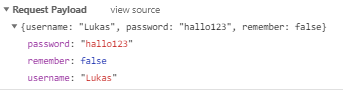
\includegraphics[scale=2.2]{images/PayloadWTForms}
	\caption{Durch WTForms ausgelöster Payload in der Browserdarstellung}
	\label{img:WTFormsPayload}
\end{figure}\\
Die \autoref{img:WTFormsPayload} stellt dar, wie die Anmeldedaten im Klartext innerhalb des Browsers zu erkennen sind. Basierend auf dieser Erkenntnis muss eine Entscheidung über den Request an den Server erfolgen. Da dieser von dem Modul ausgelöst wird, ist die Modulauswahl zu überdenken. Zur Lösung dieser Problematik wird das Modul kein Bestandteil der Chat-Funktionalität. Um die Kontrolle über Request und den Payloads zu erhalten wird im Fall der Registrierung und des Logins eigene Formulare erstellt, worauf im Weiteren detailliert eingegangen wird.

\newpage


\end{onehalfspacing}
\newpage

\bibliography{Literatur}
\newpage
%setze Anhang mit appendix
%addpart, sodass Anhang im Inhaltsverzeichnis ohne Buchstaben auftaucht
\appendix
\addpart{Anhang}




\end{document}